\documentclass[12pt]{report}
\usepackage[utf8]{inputenc}
\usepackage[russian]{babel}
%\usepackage[14pt]{extsizes}
\usepackage{listings}
\usepackage{graphicx}
\usepackage{amsmath,amsfonts,amssymb,amsthm,mathtools} 

% Для листинга кода:
\lstset{ %
language=python,                 % выбор языка для подсветки (здесь это С)
basicstyle=\small\sffamily, % размер и начертание шрифта для подсветки кода
numbers=left,               % где поставить нумерацию строк (слева\справа)
numberstyle=\tiny,           % размер шрифта для номеров строк
stepnumber=1,                   % размер шага между двумя номерами строк
numbersep=5pt,                % как далеко отстоят номера строк от подсвечиваемого кода
showspaces=false,            % показывать или нет пробелы специальными отступами
showstringspaces=false,      % показывать или нет пробелы в строках
showtabs=false,             % показывать или нет табуляцию в строках
frame=single,              % рисовать рамку вокруг кода
tabsize=2,                 % размер табуляции по умолчанию равен 2 пробелам
captionpos=t,              % позиция заголовка вверху [t] или внизу [b] 
breaklines=true,           % автоматически переносить строки (да\нет)
breakatwhitespace=false, % переносить строки только если есть пробел
escapeinside={\#*}{*)}   % если нужно добавить комментарии в коде
}
% Для измененных титулов глав:
\usepackage{titlesec, blindtext, color} % подключаем нужные пакеты
\definecolor{gray75}{gray}{0.75} % определяем цвет
\newcommand{\hsp}{\hspace{20pt}} % длина линии в 20pt
% titleformat определяет стиль
\titleformat{\chapter}[hang]{\Huge\bfseries}{\thechapter\hsp\textcolor{gray75}{|}\hsp}{0pt}{\Huge\bfseries}


% plot
\usepackage{pgfplots}
\usepackage{filecontents}
\usetikzlibrary{datavisualization}
\usetikzlibrary{datavisualization.formats.functions}
\begin{filecontents}{LevT.dat}
2 5
3 10
4 10
5 11
6 12
7 12
\end{filecontents}

\begin{filecontents}{DamLevT.dat}
2 6
3 11
4 12
5 14
6 18
7 17
\end{filecontents}

\begin{filecontents}{DamLevR.dat}
2 74
3 980
4 2147
5 4317
6 8111
7 14255
\end{filecontents}


\begin{document}
%\def\chaptername{} % убирает "Глава"
\begin{titlepage}
	\centering
	{\scshape\LARGE МГТУ им. Баумана \par}
	\vspace{3cm}
	{\scshape\Large Лабораторная работа №1\par}
	\vspace{0.5cm}	
	{\scshape\Large По курсу: "Анализ алгоритмов"\par}
	\vspace{1.5cm}
	{\huge\bfseries Расстояние Левенштейна\par}
	\vspace{2cm}
	\Large Работу выполнил: Чернов Даниил, ИУ7-56Б\par
	\vspace{0.5cm}
	\LargeПреподаватели:  Волкова Л.Л., Строганов Ю.В.\par

	\vfill
	\large \textit {Москва, 2019} \par
\end{titlepage}

\tableofcontents

\newpage
\chapter*{Введение}
\addcontentsline{toc}{chapter}{Введение}
\textbf{Расстояние Левенштейна} - минимальное количество операций вставки одного символа, удаления одного символа и замены одного символа на другой, необходимых для превращения одной строки в другую.

Расстояние Левенштейна применяется в теории информации и компьютерной лингвистике для:

\begin{itemize}
	\item исправления ошибок в слове
	\item сравнения текстовых файлов утилитой diff
	\item в биоинформатике для сравнения генов, хромосом и белков
\end{itemize}

Целью данной лабораторной работы является изучение метода динамического программирования на материале алгоритмов
Левенштейна и Дамерау-Левенштейна. 

Задачами данной лабораторной являются:
\begin{enumerate}
  	\item изучение алгоритмов Левенштейна и Дамерау-Левенштейна нахождения расстояния между строками;
	\item применение метода динамического программирования для матричной реализации указанных алгоритмов; 
	\item получение практических навыков реализации указанных алгоритмов: двух алгоритмов в матричной версии и одного из алгоритмов в рекурсивной версии; 
	\item сравнительный анализ линейной и рекурсивной реализаций выбранного алгоритма определения расстояния между строками по затрачиваемым ресурсам (времени и памяти); 
	\item экспериментальное подтверждение различий во временнóй эффективности рекурсивной и
нерекурсивной реализаций выбранного алгоритма определения расстояния между строками при
помощи разработанного программного обеспечения на материале замеров процессорного времени
выполнения реализации на варьирующихся длинах строк; 
	\item описание и обоснование полученных результатов в отчете о выполненной лабораторной
работе, выполненного как расчётно-пояснительная записка к работе. 
\end{enumerate}


\chapter{Аналитическая часть}
Задача по нахождению расстояния Левенштейна заключается в поиске минимального количества операций вставки/удаления/замены для превращения одной строки в другую.

При нахождении расстояния Дамерау — Левенштейна добавляется операция транспозиции (перестановки соседних символов).  
 
\textbf{Действия обозначаются так:} 
\begin{enumerate}
  	\item D (англ. delete) — удалить,
	\item I (англ. insert) — вставить,
	\item R (replace) — заменить,
	\item M(match) - совпадение.
\end{enumerate}

Пусть $S_{1}$ и $S_{2}$ — две строки (длиной M и N соответственно) над некоторым алфавитом, тогда расстояние Левенштейна можно подсчитать по следующей рекуррентной формуле:

\begin{displaymath}
D(i,j) = \left\{ \begin{array}{ll}
 0, & \textrm{$i = 0, j = 0$}\\
 i, & \textrm{$j = 0, i > 0$}\\
 j, & \textrm{$i = 0, j > 0$}\\
min(\\
D(i,j-1)+1,\\
D(i-1, j) +1, &\textrm{$j>0, i>0$}\\
D(i-1, j-1) + m(S_{1}[i], S_{2}[j])\\
),
  \end{array} \right.
\end{displaymath}

где $m(a,b)$ равна нулю, если $a=b$ и единице в противном случае; $min\{\,a,b,c\}$ возвращает наименьший из аргументов.

Расстояние Дамерау-Левенштейна вычисляется по следующей рекуррентной формуле:
		    
		     \[ D(i, j) =  \left\{
			\begin{aligned}
				&0, && i = 0, j = 0\\
		    	&i, && i > 0, j = 0\\
		    	&j, && i = 0, j > 0\\		    	
		    	&min \left\{
				\begin{aligned}
					&D(i, j - 1) + 1,\\
		            &D(i - 1, j) + 1,\\
		            &D(i - 1, j - 1) + m(S_{1}[i], S_{2}[i]), \\
		            &D(i - 2, j - 2) + m(S_{1}[i], S_{2}[i]),\\
		        \end{aligned} \right.
		        && 
				\begin{aligned}
					&, \text{ если } i, j > 0 \\
		            & \text{ и } S_{1}[i] = S_{2}[j - 1] \\
		            & \text{ и } S_{1}[i - 1] =  S_{2}[j] \\
		        \end{aligned} \\ 
		        &min \left\{
		        \begin{aligned}
		            &D(i, j - 1) + 1,\\
		            &D(i - 1, j) + 1, \\
		            &D(i - 1, j - 1) + m(S_{1}[i], S_{2}[i]),\\
		        \end{aligned} \right.  &&, \text{иначе}
			\end{aligned} \right.
			\]	
	    
		\subsection{Вывод}
		В данном разделе были рассмотрены алгоритмы нахождения расстояния Левенштейна и Дамерау-Левенштейна, который является модификаций первого, учитывающего возможность перестановки соседних символов. 




\chapter{Конструкторская часть}
\textbf{Требования к вводу:}
\begin{enumerate}
  	\item На вход подаются две строки
	\item uppercase и lowercase буквы считаются разными
\end{enumerate}
\textbf{Требования к программе:}
\begin{enumerate}
  	\item Две пустые строки - корректный ввод, программа не должна аварийно завершаться
\end{enumerate}
\section{Схемы алгоритмов}
В данной части будут рассмотрены схемы алгоритмов.


\begin{figure}[h]
\centering
\includegraphics[width=0.6\linewidth]{MatrixL.jpg}
\caption{Схема матричного алгоритма нахождения расстояния Левенштейна}
\label{fig:mpr}
\end{figure}


\begin{figure}[h]
\centering
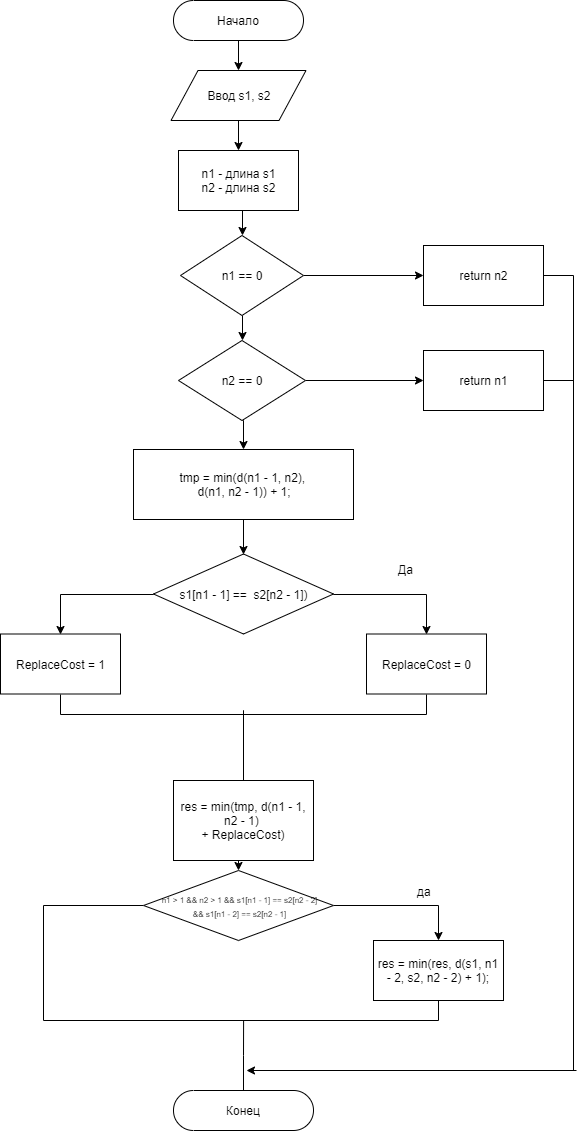
\includegraphics[width=0.75\linewidth]{RecDL.png}
\caption{Схема рекурсивного алгоритма нахождения расстояния Дамерау-Левенштейна}
\label{fig:mpr}
\end{figure}

\begin{figure}[h]
\centering
\includegraphics[width=0.75\linewidth]{MatrixDL.jpg}
\caption{Схема матричного алгоритма нахождения расстояния Дамерау-Левенштейна}
\label{fig:mpr}
\end{figure}


\chapter{Технологическая часть}
\section{Выбор ЯП}
Для реализации программ я выбрала язык программирования С\#, так имею большой опыт работы с ним. Среда разработки - Visual Studio.
Программа была разделена на несколько классов:
\begin{enumerate}
  	\item ILowensteinDistance - абстрактный родительский класс для обобщения последующих реализаций алгоритма;
	\item LowensteinDistance - класс, реализовующий поиск расстояния Левенштейна;
	\item LowensteinDamerauDistance - класс, реализовующий поиск расстояния Дамерау-Левенштейна;
	\item LowensteinDamerauRecursiveDistance - класс, реализовующий поиск рекурсивного расстояния Дамерау-Левенштейна;
	\item MainWindow - класс пользовательского интерфейса, написанный с использованием WPF;
	\item Tester - класс с тестированием методов, подсчитывающих расстояние Левенштейна.
\end{enumerate}
Ниже представлены листинги кода для перечисленных реализаций классов.

\section{Реализация алгоритма}

\begin{lstlisting}[label=some-code,caption=Абстрактный класс для последующих реализаций алгоритмов Левенштейна]
namespace LevensteinDistanceAnalysis.Core
{
    abstract class ILowensteinDistance
    {
        protected int distance;
        protected string firstWord;
        protected string secondWord;
        public int GetDistance(string firstWord, string secondWord)
        {
            this.firstWord = firstWord;
            this.secondWord = secondWord;

            if (firstWord.Length == 0 && secondWord.Length == 0)
                distance = 0;
            else if (IfJustOneWordIsEmpty())
                distance = 1;
            else
                distance = CountDistance(firstWord, secondWord);
            
            return distance;
        }
        protected bool IfJustOneWordIsEmpty()
        {
            if (firstWord.Length == 0 && secondWord.Length != 0)
                return true;
            if (firstWord.Length != 0 && secondWord.Length == 0)
                return true;
            return false;
        }
        abstract protected int CountDistance(string firstWord, string secondWord);
        override public string ToString()
        {
            return $"The distance between \"{firstWord}\" and \"{secondWord}\" is:  {distance}";
        }
    }
}
\end{lstlisting}

\begin{lstlisting}[label=some-code,caption=Класс для нахождения расстояния Левенштейна]
using System;

namespace LevensteinDistanceAnalysis.Core
{
    class LowensteinDistance : ILowensteinDistance
    {
        protected int[,] matrix;
        protected override int CountDistance(string firstWord, string secondWord)
        {
            matrix = new int[firstWord.Length + 1, secondWord.Length + 1];

            FillMatrixFirstColumnWithZeros();
            FillMatrixFirstRowWithZeros();
            FindingDistanceInMatrix();
            distance = GetResultFromMatrix();

            return distance;
        }
        protected void FindingDistanceInMatrix()
        {
            for (int i = 1; i <= firstWord.Length; i++)
            {
                for (int j = 1; j <= secondWord.Length; j++)
                {
                    GetNextElementInMatrix(i, j);
                }
            }
        }
        protected virtual void GetNextElementInMatrix(int i, int j)
        {
            int cost = (firstWord[i - 1] == secondWord[j - 1]) ? 0 : 1;

            matrix[i, j] = Math.Min(Math.Min(matrix[i - 1, j] + 1,
                                     matrix[i, j - 1] + 1),
                                     matrix[i - 1, j - 1] + cost);
        }
        protected void FillMatrixFirstColumnWithZeros()
        {
            for (int i = 0; i <= firstWord.Length; i++)
                matrix[i, 0] = i;
        }
        protected void FillMatrixFirstRowWithZeros()
        {
            for (int j = 0; j <= secondWord.Length; j++)
                matrix[0, j] = j;
        }
        protected int GetResultFromMatrix()
        {
            return matrix[firstWord.Length, secondWord.Length];
        }
        public string MatrixToString()
        {
            string distanceMatrix = "";
            for (int i = 0; i < matrix.GetLength(0); i++)
            {
                for (int j = 0; j < matrix.GetLength(1); j++)
                    distanceMatrix += matrix[i, j] + "\\t";
                distanceMatrix += "\\n";
            }
            return distanceMatrix;
        }
    }
}

\end{lstlisting}

\begin{lstlisting}[label=some-code,caption=Класс нахождения расстояния Дамерау-Левенштейна рекурсивно]
using System;

namespace LevensteinDistanceAnalysis.Core
{
    class LowensteinDamerauRecursiveDistance : ILowensteinDistance
    {
        protected override int CountDistance(string firstWord, string secondWord)
        {
            int distance = RecursiveCountDistance(firstWord, firstWord.Length, secondWord, secondWord.Length);
            return distance;
        }
        private int RecursiveCountDistance(string firstWord, int firstWordLen, string secondWord, int secondWordLen)
        {
            int cost;
            if (firstWordLen == 0) return secondWordLen;
            if (secondWordLen == 0) return firstWordLen;
            
            if (firstWord[firstWordLen - 1] == secondWord[secondWordLen - 1])
                cost = 0;
            else
                cost = 1;
            
            return Math.Min(Math.Min(RecursiveCountDistance(firstWord, firstWordLen - 1, secondWord, secondWordLen) + 1,
                            RecursiveCountDistance(firstWord, firstWordLen, secondWord, secondWordLen - 1) + 1),
                            RecursiveCountDistance(firstWord, firstWordLen - 1, secondWord, secondWordLen - 1) + cost);
        }
    }
}

\end{lstlisting}

\begin{lstlisting}[label=some-code,caption=Класс нахождения расстояния Дамерау-Левенштейна матрично]
using System;

namespace LevensteinDistanceAnalysis.Core
{
    class LowensteinDamerauDistance : LowensteinDistance
    {
        protected override void GetNextElementInMatrix(int i, int j)
        {
            int cost = (firstWord[i - 1] == secondWord[j - 1]) ? 0 : 1;

            matrix[i, j] = Math.Min(Math.Min(matrix[i - 1, j] + 1,
                                     matrix[i, j - 1] + 1),
                                     matrix[i - 1, j - 1] + cost);
            if (IfAdjacentLettersEqual(i, j))
                matrix[i, j] = Math.Min(matrix[i, j], matrix[i - 2, j - 2] + cost);
        }
        protected bool IfAdjacentLettersEqual(int i, int j)
        {
            if (i > 1 && j > 1 && firstWord[i - 1] == secondWord[j - 2] && firstWord[i - 2] == secondWord[j - 1])
                return true;
            return false;
        }
    }
}

\end{lstlisting}


\chapter{Исследовательская часть}

\section{Сравнительный анализ на основе замеров времени работы алгоритмов}

Был проведен замер времени работы каждого из алгоритмов с помощью класса StopWatch из библиотеки System.Diagnostics.
Где единицей времени является ElapsedTick - версия процессорного Тика на платформе .NET. Результаты можно увидеть в следующей таблице.

\begin{table} [h!]
\caption{Время работы алгоритмов (в тиках)}
	\begin{tabular}{|c c c c c|} 
 	\hline
	len & Lev(M) & DamLev(M) & DamLev(R) \\ [0.5ex] 
 	\hline\hline
 	2 & 5 & 6 & 74\\
 	\hline
 	3 & 10 & 11 & 980\\
 	\hline
 	4 & 10 & 12 & 2147\\
 	\hline
	5 & 11 & 14 & 4317\\
	\hline
	6 & 12 & 18 & 8111\\
	\hline
	7 & 12 & 17 & 14255\\
	\hline
	\end{tabular}
\end{table}


\begin{tikzpicture}

\begin{axis}[
    	axis lines = left,
    	xlabel={len (symbols)},
    	ylabel={time (ticks)},
    	xmin=1, xmax=7,
    	ymin=1, ymax=15000,
	legend pos=north west,
	ymajorgrids=true
]
\addplot[color=orange] table[x index=0, y index=1] {DamLevR.dat};
\addplot[color=blue, mark=square] table[x index=0, y index=1] {LevT.dat};
\addplot[color=green, mark=square] table[x index=0, y index=1] {DamLevT.dat};

\addlegendentry{DamLevR}
\addlegendentry{LevT}
\addlegendentry{DamLevT}
\end{axis}
\end{tikzpicture}


\par
Наиболее эффективными по времени при маленькой длине слова являются рекурсивные реализации алгоритмов, но как только увеличивается длина слова, их эффективность резко снижается, что обусловлено большим количеством повторных рассчетов. Время работы алгоритма, использующего матрицу, намного меньше благодаря тому, что в нем требуется только (m + 1)*(n + 1) операций заполнения ячейки матрицы. Также установлено, что алгоритм ДамерауЛевенштейна работает немного дольше алгоритма Левенштейна, т.к. в нем добавлены дополнительные проверки, однако алгоритмы сравнимы по временной эффективности.


\section{Сравнительный анализ на основе замеров потребляемой памяти алгоритмов}
\par Для проведения анализа замерим потребляемую память у разных реализаций алгоритма. Все измерения представлены в байтах и представлены в следующих таблицах.

\begin{table} [h!]
\centering
\caption{Потребляемая память структурами данных в алгоритме нахождения расстояния Левенштейна}
	\begin{tabular}{|c c c|} 
 	\hline
	Структура данных & Длина 4 символа & Длина 1000 символов\\ [0.8ex] 
 	\hline\hline
 	Матрица & 480 & 8064096\\
 	\hline
 	Две вспомогательные переменные (int) & 56 & 56\\
 	\hline
	Два счетчика (int) & 56 & 56\\
	\hline
	Передача параметров & 106 & 2098\\
	\hline
	Cумма данных & 698 & 8066306\\
	\hline
	\end{tabular}
\end{table}

\begin{table} [h!]
\centering
\caption{Потребляемая память структурами данных в алгоритме нахождения расстояния Дамерау-Левенштейна}
	\begin{tabular}{|c c c|} 
 	\hline
	Структура данных & Длина 4 символа & Длина 1000 символов\\ [0.8ex] 
 	\hline\hline
 	Матрица & 480 & 8064096\\
 	\hline
 	Три вспомогательные переменные (int) & 84 & 84\\
 	\hline
	Два счетчика (int) & 56 & 56\\
	\hline
	Передача параметров & 106 & 2098\\
	\hline
	Cумма данных & 726 & 8066334\\
	\hline
	\end{tabular}
\end{table}

\begin{table} [h!]
\centering
\caption{Потребляемая память структурами данных в рекурсивном алгоритме нахождения расстояния Дамерау-Левенштейна}
	\begin{tabular}{|c c c|} 
 	\hline
	Структура данных & Длина 4 символа & Длина 1000 символов\\ [0.8ex] 
 	\hline\hline
 	Пять переменных для подсчета IDTR & 140 * 4 = 560 & 140 * 1000 = 140000\\
 	\hline
	Передача параметров & 106 * 4/2 = 212 & 2098 * 1000/2 = 1049000\\
	\hline
	Cумма данных & 772 & 1189000\\
	\hline
	\end{tabular}
\end{table}


\par
Таким образом, рекурсивный алгоритм занимает примерно одинаковое кол-во памяти при маленькой длине строк, и значительно выигрывает при строках большего размера.


\section{Тестирование}

\par
Тестирование проводилось в виде Unit Тестов, то есть тестов отдельных компонентов (методов) вычисляющих расстояние Левенштейна.
Было написано 15 тестовых случаев по 5 различных случаев для каждой из трёх реализаций. Тестовые методы рассматривают такие случаи:
\begin{enumerate}
  	\item даны две пустые строки
	\item дана одна пустая а вторая непустая строки
	\item даны две одинаковые строки
	\item даны две строки с одной различной буквой
	\item даны две пустые строки, где необходимо сделать перестановку
\end{enumerate}
Примеры тестов можно увидеть в следующей таблице.

\begin{table} [h!]
\caption{Таблица тестовых данных}
	\begin{tabular}{|c c c c c|} 
 	\hline
	№ & Первое слово & Второе слово & Ожидаемый результат & Полученный результат \\ [0.8ex] 
 	\hline\hline
 	1 &  &  & 0 0 0 & 0 0 0\\
 	\hline
 	2 & kot & skat & 2 2 2 & 2 2 2\\
 	\hline
	3 & kate & ktae & 2 1 1 & 2 1 1\\
	\hline
	4 & abacaba & aabcaab & 4 2 2 & 4 2 2\\
	\hline
	5 & sobaka & sboku & 3 3 3 & 3 3 3\\
	\hline
	6 & qwerty & queue & 4 4 4 & 4 4 4\\
	\hline
	7 & apple & aplpe & 2 1 1  & 2 1 1\\
	\hline
	8 &  & cat & 3 3 3 & 3 3 3\\
	\hline
	9 & parallels &  & 9 9 9 & 9 9 9\\
	\hline
	10 & bmstu & utsmb & 4 4 4 & 4 4 4\\
	\hline
	\end{tabular}
\end{table}



\chapter*{Заключение}
\addcontentsline{toc}{chapter}{Заключение}
Был изучен метод динамического программирования на материале алгоритмов Левенштейна и Дамерау-Левенштейна.
Также изучены алгоритмы Левенштейна и Дамерау-Левенштейна нахождения расстояния между строками, получены практические навыки раелизации указанных алгоритмов
в матричной  и рекурсивных версиях. 
Экспериментально было подтверждено различие во временной эффективности рекурсивной и нерекурсивной реализаций выбранного алгоритма определения 
расстояния между строками при помощи разработаного программного обеспечения на материале замеров процессорного времени выполнения 
реализации на варьирующихся длинах строк. 
В результате исследований я пришел к выводу, что матричная реализация данных алгоритмов заметно выигрывает по времени при росте 
длины строк, следовательно более применима в реальных проектах.


\end{document}